\documentclass[a4paper, 11pt, oneside]{article}

\usepackage[utf8]{inputenc}
\usepackage[T1]{fontenc}
\usepackage[french]{babel}
\usepackage{array}
\usepackage{shortvrb}
\usepackage{listings}
\usepackage[fleqn]{amsmath}
\usepackage{amsfonts}
\usepackage{fullpage}
\usepackage{enumerate}
\usepackage{graphicx}             % import, scale, and rotate graphics
\usepackage{subfigure}            % group figures
\usepackage{alltt}
\usepackage{url}
\usepackage{indentfirst}
\usepackage{eurosym}
\usepackage{listings}
\usepackage{color}
\usepackage[table,xcdraw,dvipsnames]{xcolor}

% Change le nom par défaut des listing
\renewcommand{\lstlistingname}{Extrait de Code}

% Change la police des titres pour convenir à votre seul lecteur
\usepackage{sectsty}
\allsectionsfont{\sffamily\mdseries\upshape}
% Idem pour la table des matière.
\usepackage[nottoc,notlof,notlot]{tocbibind}
\usepackage[titles,subfigure]{tocloft}
\renewcommand{\cftsecfont}{\rmfamily\mdseries\upshape}
\renewcommand{\cftsecpagefont}{\rmfamily\mdseries\upshape}

\definecolor{mygray}{rgb}{0.5,0.5,0.5}
\newcommand{\coms}[1]{\textcolor{MidnightBlue}{#1}}

\lstset{
    language=C, % Utilisation du langage C
    commentstyle={\color{MidnightBlue}}, % Couleur des commentaires
    frame=single, % Entoure le code d'un joli cadre
    rulecolor=\color{black}, % Couleur de la ligne qui forme le cadre
    stringstyle=\color{RawSienna}, % Couleur des chaines de caractères
    numbers=left, % Ajoute une numérotation des lignes à gauche
    numbersep=5pt, % Distance entre les numérots de lignes et le code
    numberstyle=\tiny\color{mygray}, % Couleur des numéros de lignes
    basicstyle=\tt\footnotesize,
    tabsize=3, % Largeur des tabulations par défaut
    keywordstyle=\tt\bf\footnotesize\color{Sepia}, % Style des mots-clés
    extendedchars=true,
    captionpos=b, % sets the caption-position to bottom
    texcl=true, % Commentaires sur une ligne interprétés en Latex
    showstringspaces=false, % Ne montre pas les espace dans les chaines de caractères
    escapeinside={(>}{<)}, % Permet de mettre du latex entre des <( et )>.
    inputencoding=utf8,
    literate=
  {á}{{\'a}}1 {é}{{\'e}}1 {í}{{\'i}}1 {ó}{{\'o}}1 {ú}{{\'u}}1
  {Á}{{\'A}}1 {É}{{\'E}}1 {Í}{{\'I}}1 {Ó}{{\'O}}1 {Ú}{{\'U}}1
  {à}{{\`a}}1 {è}{{\`e}}1 {ì}{{\`i}}1 {ò}{{\`o}}1 {ù}{{\`u}}1
  {À}{{\`A}}1 {È}{{\`E}}1 {Ì}{{\`I}}1 {Ò}{{\`O}}1 {Ù}{{\`U}}1
  {ä}{{\"a}}1 {ë}{{\"e}}1 {ï}{{\"i}}1 {ö}{{\"o}}1 {ü}{{\"u}}1
  {Ä}{{\"A}}1 {Ë}{{\"E}}1 {Ï}{{\"I}}1 {Ö}{{\"O}}1 {Ü}{{\"U}}1
  {â}{{\^a}}1 {ê}{{\^e}}1 {î}{{\^i}}1 {ô}{{\^o}}1 {û}{{\^u}}1
  {Â}{{\^A}}1 {Ê}{{\^E}}1 {Î}{{\^I}}1 {Ô}{{\^O}}1 {Û}{{\^U}}1
  {œ}{{\oe}}1 {Œ}{{\OE}}1 {æ}{{\ae}}1 {Æ}{{\AE}}1 {ß}{{\ss}}1
  {ű}{{\H{u}}}1 {Ű}{{\H{U}}}1 {ő}{{\H{o}}}1 {Ő}{{\H{O}}}1
  {ç}{{\c c}}1 {Ç}{{\c C}}1 {ø}{{\o}}1 {å}{{\r a}}1 {Å}{{\r A}}1
  {€}{{\euro}}1 {£}{{\pounds}}1 {«}{{\guillemotleft}}1
  {»}{{\guillemotright}}1 {ñ}{{\~n}}1 {Ñ}{{\~N}}1 {¿}{{?`}}1
}
\newcommand{\tablemat}{~}

%%%%%%%%%%%%%%%%% TITRE %%%%%%%%%%%%%%%%
% Complétez et décommentez les définitions de macros suivantes :
\newcommand{\intitule}{Multiplicité INFO0947}
\newcommand{\GrNbr}{21}
\newcommand{\PrenomUN}{Maxime}
\newcommand{\NomUN}{Deravet}
\newcommand{\PrenomDEUX}{Luca}
\newcommand{\NomDEUX}{Matagne}
\renewcommand{\tablemat}{\tableofcontents}

%%%%%%%% ZONE PROTÉGÉE : MODIFIEZ UNE DES DIX PROCHAINES %%%%%%%%
%%%%%%%%            LIGNES POUR PERDRE 2 PTS.            %%%%%%%%
\title{INFO0947: \intitule}
\author{Groupe \GrNbr : \PrenomUN~\textsc{\NomUN}, \PrenomDEUX~\textsc{\NomDEUX}}
\date{}
\begin{document}
\maketitle
\newpage
\tablemat
\newpage
%%%%%%%%%%%%%%%%%%%% FIN DE LA ZONE PROTÉGÉE %%%%%%%%%%%%%%%%%%%%

%%%%%%%%%%%%%%%% RAPPORT %%%%%%%%%%%%%%%
% Écrivez votre rapport ci-dessous.


\section{spécification du module "multiplicité"}

\begin{lstlisting}[caption={Spécifications}]
/**
 * multiplicite
 *
 *  @pre : N > 0, T est un tableau d'entier de taille
 *
 *  @post: max contient le maximum du tableau
 *
 *  @return: le nombre d'occurence de max
 *
**/


int multiplicite(int *T, const int N, int *max);

\end{lstlisting}



\section{Nos Sous-Problèmes}

\subsection{SP 1: Obtenir le max du tableau}

La notation du sous-problème consistant à obtenir le maximun du tableau est la suivante:
MaximumSSTab(T,i,j,N)$ \equiv 0 \le i \le j < N$

\bigskip
Dans ce sous problème, nous allons introduire notre boucle while. Voci donc l'invariant de boucle qui nous a permis d'écrire notre code:

\centering
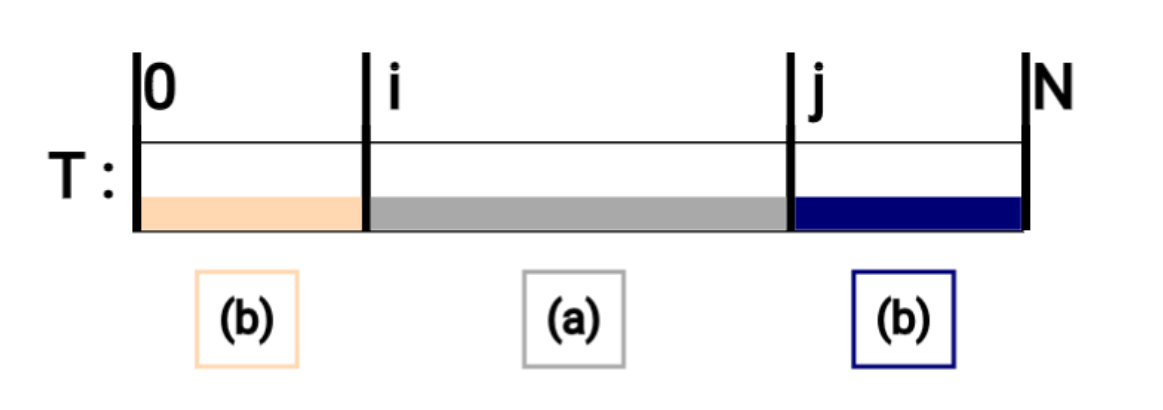
\includegraphics[scale=0.2]{loopMulti.png}

b = Maximum trouvé ||
a = Éventuel maximum à trouver

\flushleft
\setlength{\parindent}{0.5cm}

L'invariant formel qui découle de cet invariant graphique est naturellement en lien avec la notation de notre sou-problème(en début de sous-section), le voici:

max=MaximumSSTab $\land$ $ 0 \le i \le j < N$

Fonction de terminaison:

\subsection{SP 2: Compter le nombre d'occurence du max}

Il est important de comprendre que ce sous problème n'est pas la suite du premier mais est bl et bien inclus dans le premier sous-problème. On va donc faire attention à exécuter les instructions de ce sous problème À CHAQUE ITÉRATION DE NOTRE BOUCLE (dont l'invariant est rappelé dans  le SP1).

Le principe va être de créer une variable "occurence" et d'incrémenter cette variable de 1 à chaque fois qu'un même maximum est détecté. Dans le cas ou un nouveau maximum est trouvé, cette variable est naturellement ramenée à 1.



\section{Vérification de la complexité}





\section{Code}
\subsection{multiplicite.h}
\begin{lstlisting}[caption={Header}]

#ifndef __MULTI__
#define __MULTI__

/**
 * multiplicite
 *
 *  @pre : N > 0, T est un tableau d'entier de taille
 *
 *  @post: max contient le maximum du tableau
 *
 *  @return: le nombre d'occurence de max
 *
**/


int multiplicite(int *T, const int N, int *max);


#endif


\end{lstlisting}

\subsection{main.c}
\begin{lstlisting}[caption={Main}]

#include <stdio.h>
#include "multiplicite.h"



int main(){

   int T[10] = {16, 16,10, 16,160, 16, 16, 16, 16, 16};
   int max = 0;
   multiplicite(T,10,&max);
   printf("%d - %d\n",multiplicite(T,10,&max),max );



}

\end{lstlisting}

\newpage
\subsection{multiplicite.c}
\begin{lstlisting}[caption={multiplicite.c}]

#include "multiplicite.h"
#include <assert.h>

int multiplicite(int *T, const int N, int *max){

   assert (N>0);
   assert (T!=0);

   int i = 0;
   int j = N-1;
   int temp = 0;
   int occurence = 0;
   int nbri;
   int nbrj;
   int maxi;


   while (i <= j){
      nbri = T[i];
      nbrj = T[j];


      //Nombre le plus grand entre les deux valeurs actuelles

      if (i!=j){
         if (nbri > nbrj){
            temp = nbri;
         }//fin if i>j

         else{
            temp = nbrj;
         }//fin else
      }
      else
      temp = nbri;


     //Changement du maximum et du nombre d'occurence

      if (i ==0){ //Premier tour de boucle
         maxi = temp;
         if ((nbri == nbrj)&&(i!=j))
            occurence = 2;
         else
            occurence = 1;
      }//fin if i ==0

      if (maxi < temp){ //si le nouveau nombre est plus grand, changement et reinitialisation de l'occurences
         maxi = temp;
         if ((nbri == nbrj)&&(i!=j)) // si les deux valeurs sont égale et qu'on regarde deux valeur différente => (Occurence ==2)  sinon occurence ==1
            occurence = 2;
         else
            occurence = 1;
      }//fin if max<temp


      else if ((maxi == temp) && (i!=0)){//Si le nouveau nombre est égal, augmentation de l'occurence

         if ((nbri == nbrj)&&(i!=j)) // si les deux valeurs sont égale et qu'on regarde deux valeur différente => (Occurence +2)  sinon occurence +1
            occurence += 2;
         else
            occurence += 1;
      }//fin if maxi == temp


    //incrémentation des compteurs
      i++;
      j--;



   }//fin while

   *max = maxi;

   return occurence;

}//fin multiplicite


\end{lstlisting}




\newpage
\section{Insérer du code Latex}

\begin{lstlisting}[caption={Un programme tout simple}]
int main(void)
{
	// Les commandes Latex sont permises dans les commentaires sur une ligne. Exemple : $x_i \leq a ^b$
	printf("Bonjour tout le monde !");
	/*
	Dans les commentaires sur plusieurs lignes, elles doivent être entourées
	de symboles définis par l'option « escapeinside » de \lstset
	(>\coms{$\sum_{i = 1}^N 1 = N$}<)
	La commande « \coms » permet de colorer correctement le code latex ajouté.
	Les accents et tous les autres diacritiques sont permis : àÀçÇéÉèÈêÊœŒ...
	*/
	return 1; (>\label{code:ret}<)
}
\end{lstlisting}

Il est possible de faire référence à la ligne \ref{code:ret} de l'extrait de code.

\section{Dessiner un tableau}

Comme mentionné sur le forum «~\emph{eCampus > Forum : Projets -- Informations générales > Thème : Dessine-moi un invariant !}~», il est possible de dessiner facilement des tableaux. Le résultat de l'exemple donné sur le forum eCampus est visible dans la figure \ref{fig:exemple}.

\begin{figure}[!h]
\centering
\begin{tabular}{l|llr|ll|l}
 & 0 &  & \multicolumn{1}{r|}{i-1} & i &  & N \\ \cline{2-6}
t: & \cellcolor[HTML]{FFCC67} & \cellcolor[HTML]{FFCC67}. > 0 & \cellcolor[HTML]{FFCC67} &  &  &  \\ \cline{2-6}
\end{tabular}
\caption{Voici le tableau de l'exemple}
\label{fig:exemple}
\end{figure}

\section{Autres conseils}

\subsection{Utilisez les bons opérateurs}

Voir la table \ref{table:op}.

\begin{table}[!h]
\centering
\begin{tabular}{l c}
Nom & Op \\
\hline
ET & $\land$ \\
OU & $\lor$ \\
Quantification universelle & $\forall$ \\
Quantification existentielle & $\exists$ \\
\end{tabular}
\caption{Opérateurs les plus usuels en logique}
\label{table:op}
\end{table}

\subsection{Trouver un symbole précis}

Voir ce site : \url{http://detexify.kirelabs.org/classify.html}. Il suffit de dessiner le symbole dont vous avez besoin et le site trouvera (normalement) la bonne commande à taper (ainsi que le package à éventuellement inclure si besoin est).

\subsection{N'oubliez pas de relire le résultat produit par la compilation}

\end{document}
